\title{CS 523. Complex Adaptive Systems Final Project\\ Allocation of Tasks on Real-Time Multiprocessor Systems using Genetic Algorithms}

\author{ Oscar Mondragon, and  
Amanda Minnich \\
Computer Science Department\\
University of New Mexico\\
{\rm \{omondrag, aminnich\}@cs.unm.edu  }\\
%copy the following lines to add more authors
% \and
% {\rm Name}\\
%Name Institution
} % end author
          
\date{May 1, 2013}

\documentclass[11pt]{article}
\usepackage{graphicx,float,wrapfig}
\usepackage[margin=0.92in]{geometry}
\usepackage{wrapfig}
\usepackage{url}
\usepackage{tabularx}
\usepackage{siunitx}
\usepackage{setspace}
\usepackage{cite}
\singlespacing


\begin{document}
\maketitle
\doublespacing

\section{Author Contributions}
Both Mondragon and Minnich worked extensively on the code, meeting daily to work on all steps of the coding process. Mondragon spent additional time debugging, since he was more familiar with C. Mondragon also generated the smaller chromosome and tested it in Palacios Virtual Machine Monitor. Minnich generated the figures and tables. They each ran half of the experiments. Mondragon wrote the Introduction, the methods and results of the Palacios experiment and the Related Work, and Minnich wrote the Methods, Results, and Conclusion.

\section{Introduction}

For this project, we wrote a genetic algorithm that evolves ideal parameters for task allocation on real-time multiprocessor systems. This allocation problem is one with a high computational complexity solution~\cite{Mondragon:13}. There are two approaches to solving this problem: the partitioning strategy, in which all the instances of a task are allocated to a single processor, and the global strategy, in which any instance of a task can migrate among processors when required~\cite{Lopez:04}. The multiprocessor maximum utilization bound depends on the allocation algorithm used. For our project, we will be using the partitioning approach.  Since this allocation problem is NP hard, some approximate solutions have been proposed which include the Worst Fit (WF), First Fit (FF), Next Fit (NF), and Best Fit (BF) heuristics~\cite{Zapata:05}. 

Allocation of tasks is followed by scheduling of these tasks in a real time multiprocessor system. Scheduling is also a complex problem, and algorithms such as Rate Monotonic Scheduling (RM) and Earliest Deadline First Scheduling (EDF) ~\cite{Dall:78} have been proposed. The optimal allocation of tasks depends on what kind of scheduling algorithm one wants to use. For this project, we want to prepare an optimal allocation of tasks for the EDF scheduler. This scheduler uses dynamically calculated priorities as scheduling criteria to choose what task will be scheduled next. These priority values are calculated based on the deadlines of the tasks that are in the run queue. Tasks with earliest deadline will receive higher priorities. A period (T) and a slice (C) are associated with each task. The period is defined as the amount of time the task may receive a CPU allocation, and the slice is the minimum amount of time received for the task during each period~\cite{Chung:73}. The portion of CPU used for a task is $\frac{C}{T}$. Therefore, the utilization factor of a CPU is given by: 

\begin{center}
$U = \sum_{i=1}^{n} \frac{C_{i}}{T_{i}}$ , where n is the number of tasks allocated on a CPU.
\end{center}

Allocation and scheduling have a direct application to Virtual Machine Monitors (VMMs), where virtual cores need to be allocated to and scheduled on physical cores. In this problem a variable called the time dilation factor (TDF) also affects allocation. Time dilation allows the perceived availability of resources of a virtual machine to be changed by altering the real time by a factor, called the time dilation factor. This provides for the slowing down or speeding up the passage of time detected by a guest operating system ~\cite{Gupta:06}. Slowing down the system has the effect of making the external world appear sped up. For example, if you have a TDF of 10, for 10 seconds of real time you have 1 second in the guest system, so the guest system recieves more events from the external world per unit time. The TDF is defined as $\frac{real time}{virtual time}$. During allocation, the following formulas relating to the TDF must always be satisfied:

\begin{center}
%$ \frac{1}{TDF} \cdot \sum_{n}^{i=1} \frac{C_{i}}{T_{i}} \leq U_{MAX}$ 
$\frac{U}{TDF} \leq U_{MAX} \leq 1$ and
$\frac{\sum_{i=1}^{n} F_{VCPUi} }{F_{PCPU}} \leq TDF$
\end{center}
\begin{flushleft}
where $F_{PCPU}$ is the speed of a physical CPU and $F_{VCPUi}$ is the speed of a virtual core allocated to that physical CPU. 
\end{flushleft}
Having these constraints adds a level of complexity to our genetic algorithm, since they are not simply boundary checking. Because they involve parameters from different entities, there are more complex constraint relationships than there have been in the genetic algorithms we have written previously.

Since the goal is to use our resources as efficiently as possible while obeying the above constraints, we define our fitness function as

\begin{center}

$fitness = \frac{\sum_{i=1}^{n} \frac{U_{achieved_i}}{U_{max_i}}}{TDF \cdot n}$

\begin{flushleft}
where $n =$ number of physical cores, 

$U_{achieved_{i}} =$ Achieved utilization for physical core i, and

$U_{max_{i}} =$ Maximum utilization for physical core i.
\end{flushleft}

\end{center}

This fitness function measures how close to full each of our physical CPUs are. We plan to always provide enough virtual cores to saturate the available physical cores. 

Since optimizing the allocation of tasks on real-time multiprocessors systems is quite complex, this seems be an  ideal problem to which to apply a genetic algorithm. There are a variety of parameters to be optimized, and we need to explore the parameter space, but to do so exhaustively would take exponential time. By encoding a fitness function related to the efficient use of our multiprocessor resources, we can use the genetic algorithm to evolve parameters that (roughly) maximize this value.

\section{Related Work}

Other works like~\cite{Shahid94,Wu04anincremental,Omara2010} have used genetic algorithms for solving the CPU allocation problem. Our work differs from these approaches in two main aspects. The first is the scope of our algorithm, which is oriented specifically towards optimizing the allocation problem of systems using a real time scheduling mechanism, more specifically towards solving this problem in the context of VMMs, where parameters such as the TDF play an important role in the allocation process. The second is the complexity of our chromosome, which includes multiple parameters from different entities that need to be optimized and which has to meet constraints imposed for the scheduling algorithm in order to produce a legal allocation result.


\section{Methods}

Our program consits of around 900 lines of C code. We chose that programming language because it easily interfaces with existing virtualization software. We input the number of machines in the population, the number of generations for the algorithm to run, the number of physical cores and the number of virtual cores in the virtual machine. Our experiments were all run with 50 physical cores and 650 virtual cores. We select random values in a fixed range for the maximum utilization value for each physical core and the CPU speed for both the physical and virtual cores. These values are fixed across the different machines in the population: for example in every machine physical core number 1 will have the same (initially random) maximum utilization and speed values. Our chromosome consists of a TDF for the virtual machine, slice and period values for every core of every virtual machine, and an allocation matching of a virtual core to a physical core for every virtual core. We created structs to represent physical cores, virtual cores, the virtual machine, an overall machine which corresponds to an individual in the population, and the population itself, which had 100 individuals for all experiments. This was necessary because of the hierarchical nature of this system. 

While writing this program, we took inspiration from the genetic algorithms from Project 2, but due to the nature of the problem modifications in implementation were necessary. Like standard genetic algorithms, our chromosome parameters receive random initial values, and over the course of the experiment they undergo selection, crossover, and mutation, along with a fitness evaluation at the end of each round. We used tournament selection, with and without elitism. When elitism was present, the elite individual did not undergo crossover or mutation. That individual could however be picked during selection again to participate in these processes. We implemented standard 1-pt crossover, where a random crossover point is picked and two parents swap chromosome values at this point. For our mutation function, we re-assigned random parameter values for the virtual core parameters. We did not mutate the TDF, due to difficulties with constraint checking. This did not seem to have a large effect on the outcome of the experiment. 

As described above, certain constraints had to be checked each time the chromosome was modified. If these constraints were not met, the changes had to be rolled back and attempted again. We included a counter in our crossover and mutation functions, as we found that sometimes no new satisfying parameters could be found, especially further along in the evolution process. The constraints described above involved parameters from different structs, for example the TDF is a virtual machine parameter and UMax is a physical core parameter. This interconnectedness, as well as the hierarchical nature of these systems, added considerable complexity to the implementation of our genetic alorithm. 

Once we got the genetic algorithm working, we ran 12 experiments to explore high and low mutation and crossover rates, as well as to better understand the effects of elitism. We generated CSV files and created plots with MATLAB. 

We also did a smaller-scale run of our genetic algorithm and tested the top-performing chromosome values in the Palacios Virtual Machine Monitor, which is a free software package that Mondragon currently works with~\cite{Mondragon:13}. As mentioned above, our genetic algorithm attempts to generate a suitable allocation configuration oriented to maximize the utilization of the physical CPUs when the Earliest Deadline Scheduler (EDF) is used. This scheduler has been previously implemented in Palacios VMM as part of Mondragon's research and was used to validate our results.

We kept all of the same parameters of the previous test cases, but reduced the number of physical cores to 3 and the number of virtual cores to 6. Both mutation and crossover rates were set to 0.5 and elitism was used. For this experiment the 2.6.37 linux kernel was compiled into a bootable ISO image. This image was installed whithin a QEMU~\cite{Bellard:2005} emulated machine, and Palacios was executed embedded in that linux distribution. In QEMU options, 3 physical cores were specified and the amount of RAM memory was set to 2048 MB. To get the palacios logs outside QEMU, the option -serial was used. For the guest configuration, the parameters specified in the chromosome, such as TDF, slice, period, and allocated cpu (target CPU) were written in the VM XML config file. This XML file was used to generate the VM by using the guest\_creator tool provided by Palacios. Given to the complexity of the installation, and configuration of Palacios VMM and its VM guests, the Palacios code is not provided. The complete installation and setting was done on Mondragon's personal computer; if required, it can be shown in operation on that machine. In addition, the Palacios log file is provided in our turned in materials.

\section{Results}

The results for the performance of this program were quite positive, even for a large number of virtual cores. There was substantial improvement in fitness values no matter what the set of algorithm parameters were, with average fitness values increasing from 0.2 to 0.4, and the best fitness values increasing from 0.4 to 0.8. Since the purpose of genetic algorithms is to generate at least one high fitness individual, we feel that the high fitness value reached by the best individuals is quite significant, even if there was an overall lower change in average fitness values. Furthermore, this evolution happened very early on. We ran 50 generations in each experiment for thoroughness, but most of the evolution happened by 10 generations. This makes this algorithm more practical for actual use, as 10 generations run very quickly. Thus it is reasonable to hope that researchers could use this code to assist in virtual core allocation, as it works well and runs quickly. 

It is clear from the figures~\ref{fig:fig1} and~\ref{fig:fig2} that crossover and mutation rates do not have a large effect on the efficacy of this genetic algorithm. This suggests that the fitness landscape of this type of allocation is smooth, with a distinct maximum. 

\begin{figure}[H]
 \centering
  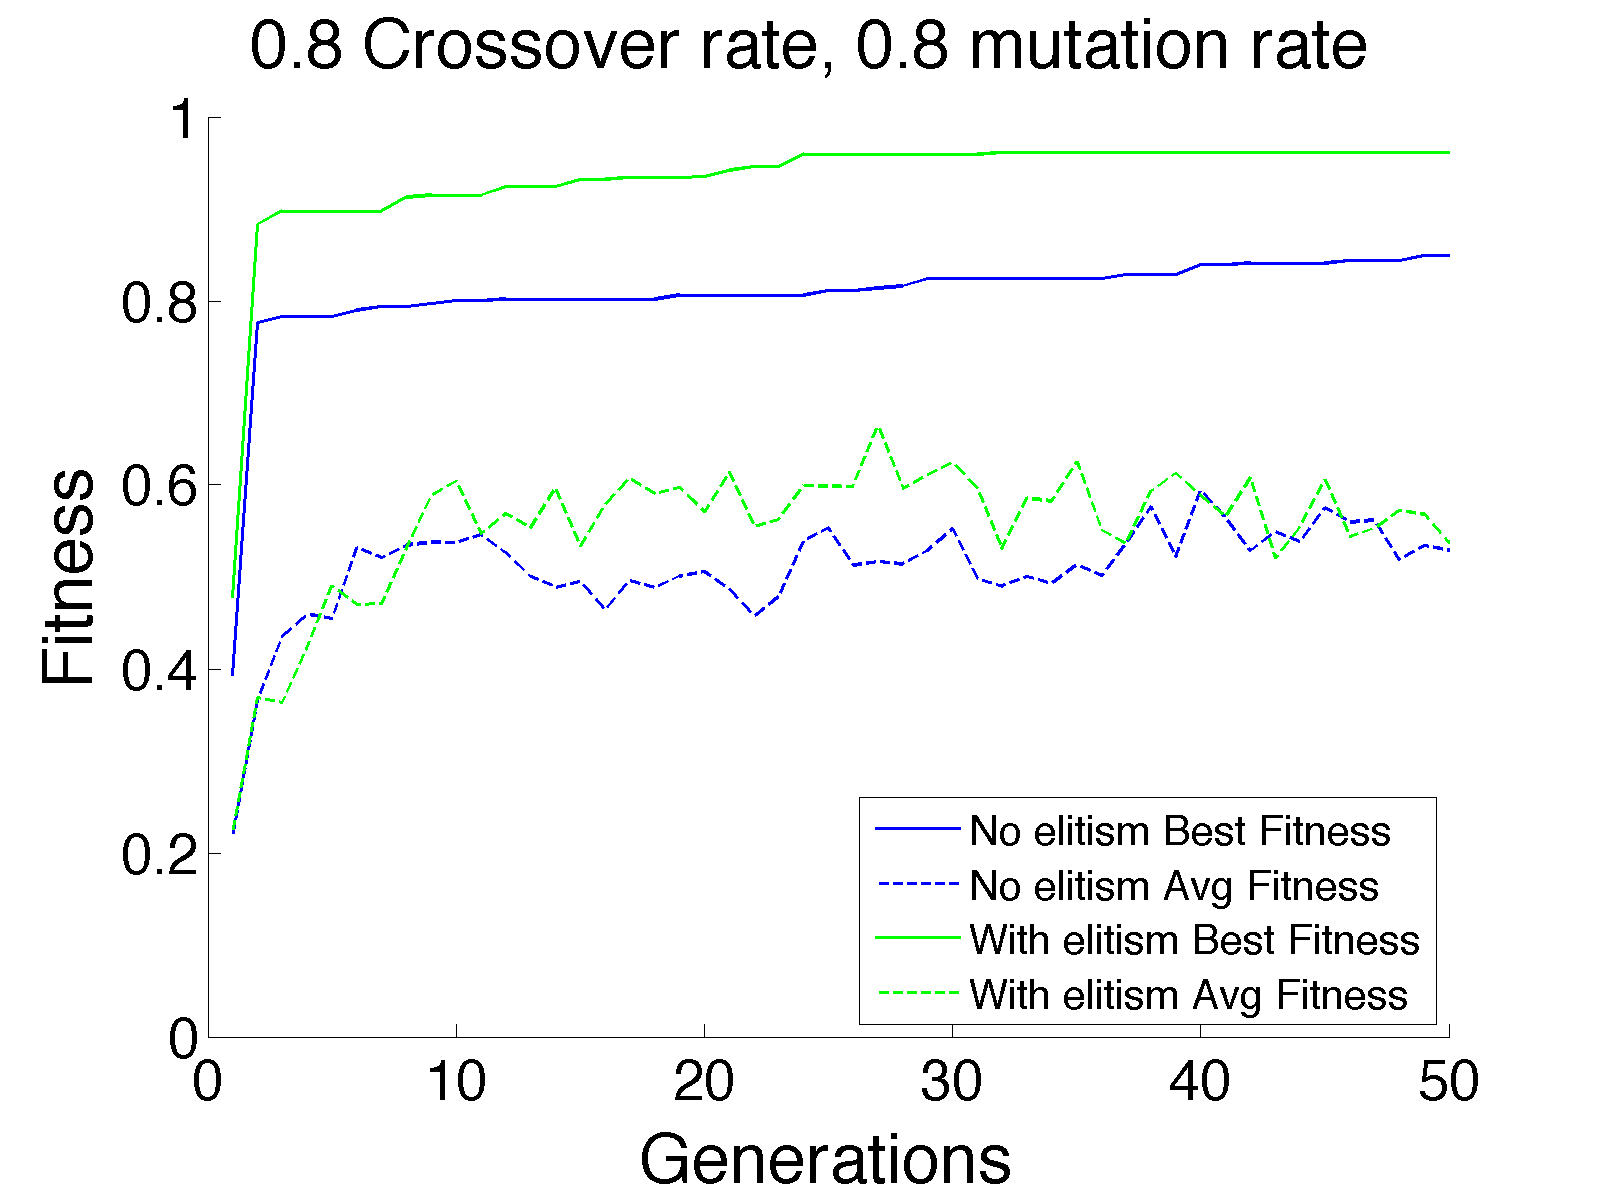
\includegraphics[width=0.6\textwidth,height=0.2\textheight]{figures/fitness08mut08cross.png}
  \caption{Best and average fitness curves with and without elitism with a 0.8 crossover rate and a 0.8 mutation rate}
  \label{fig:fig1}  
\end{figure} 

\begin{figure}[H]
 \centering
  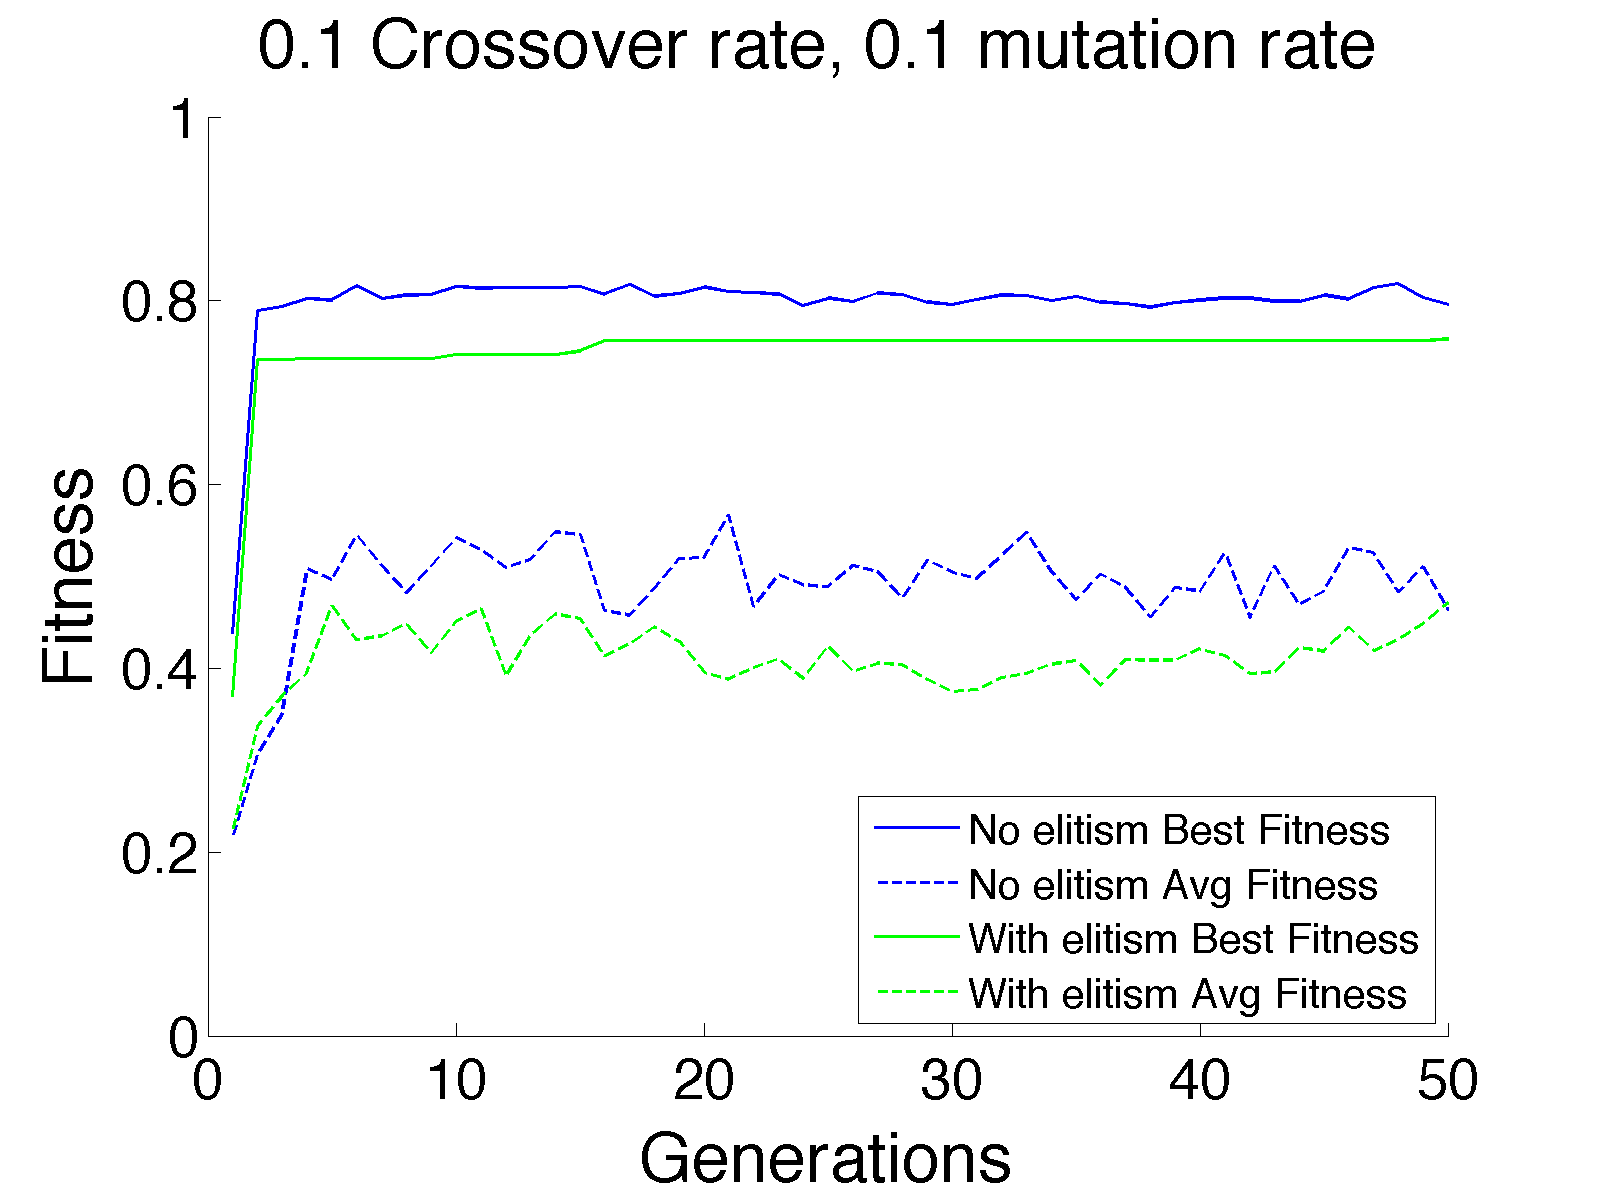
\includegraphics[width=0.6\textwidth,height=0.2\textheight]{figures/fitness01mut01cross.png}
  \caption{Best and average fitness curves with and without elitism with a 0.1 crossover rate and a 0.1 mutation rate}
  \label{fig:fig2}  
\end{figure}

In genetic algorithms, elitism and mutation have a clear relationship: if the mutation rate is low, elitism is often unnecessary, but if it is high, it is quite important. we wanted to explore this relationship, so we ran two experiments, one with a high crossover rate and no mutation (See Figure ~\ref{fig:fig3}), and one with a high mutation rate and no crossover (See Figure ~\ref{fig:fig4}). When there is no mutation, elitism seems to be detrimental, with a best fitness value of just above 0.6, while the run without elitism gets to around 0.8. 

With a high mutation rate, elitism does indeed prove essential. Although initially the run without elitism is performing better, the high mutation rate causes the best-performing chromosome to be lost, resulting in a steep drop in both the best and average fitness values.
 
\begin{figure}[H]
 \centering
  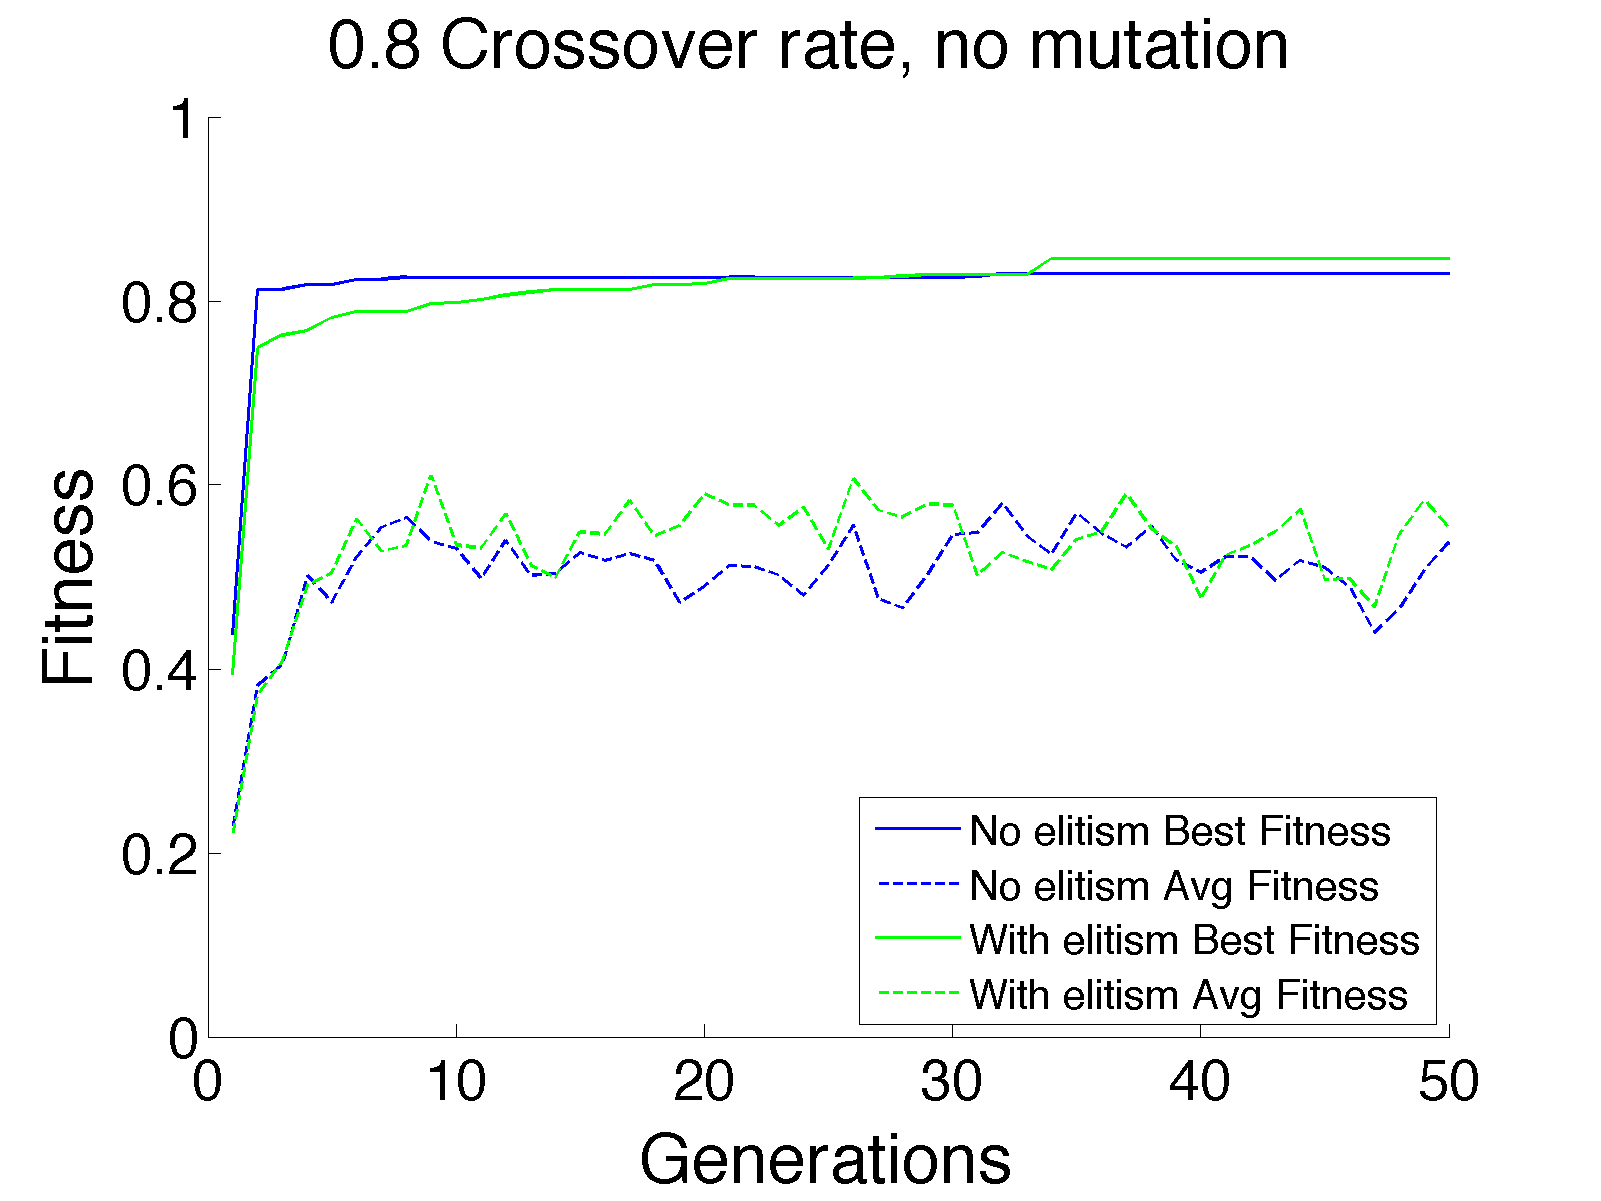
\includegraphics[width=0.6\textwidth,height=0.2\textheight]{figures/fitness0mut08cross.png}
  \caption{Best and average fitness curves with and without elitism with a 0.8 crossover rate and no mutation}
  \label{fig:fig3}  
\end{figure}

\begin{figure}[H]
 \centering
  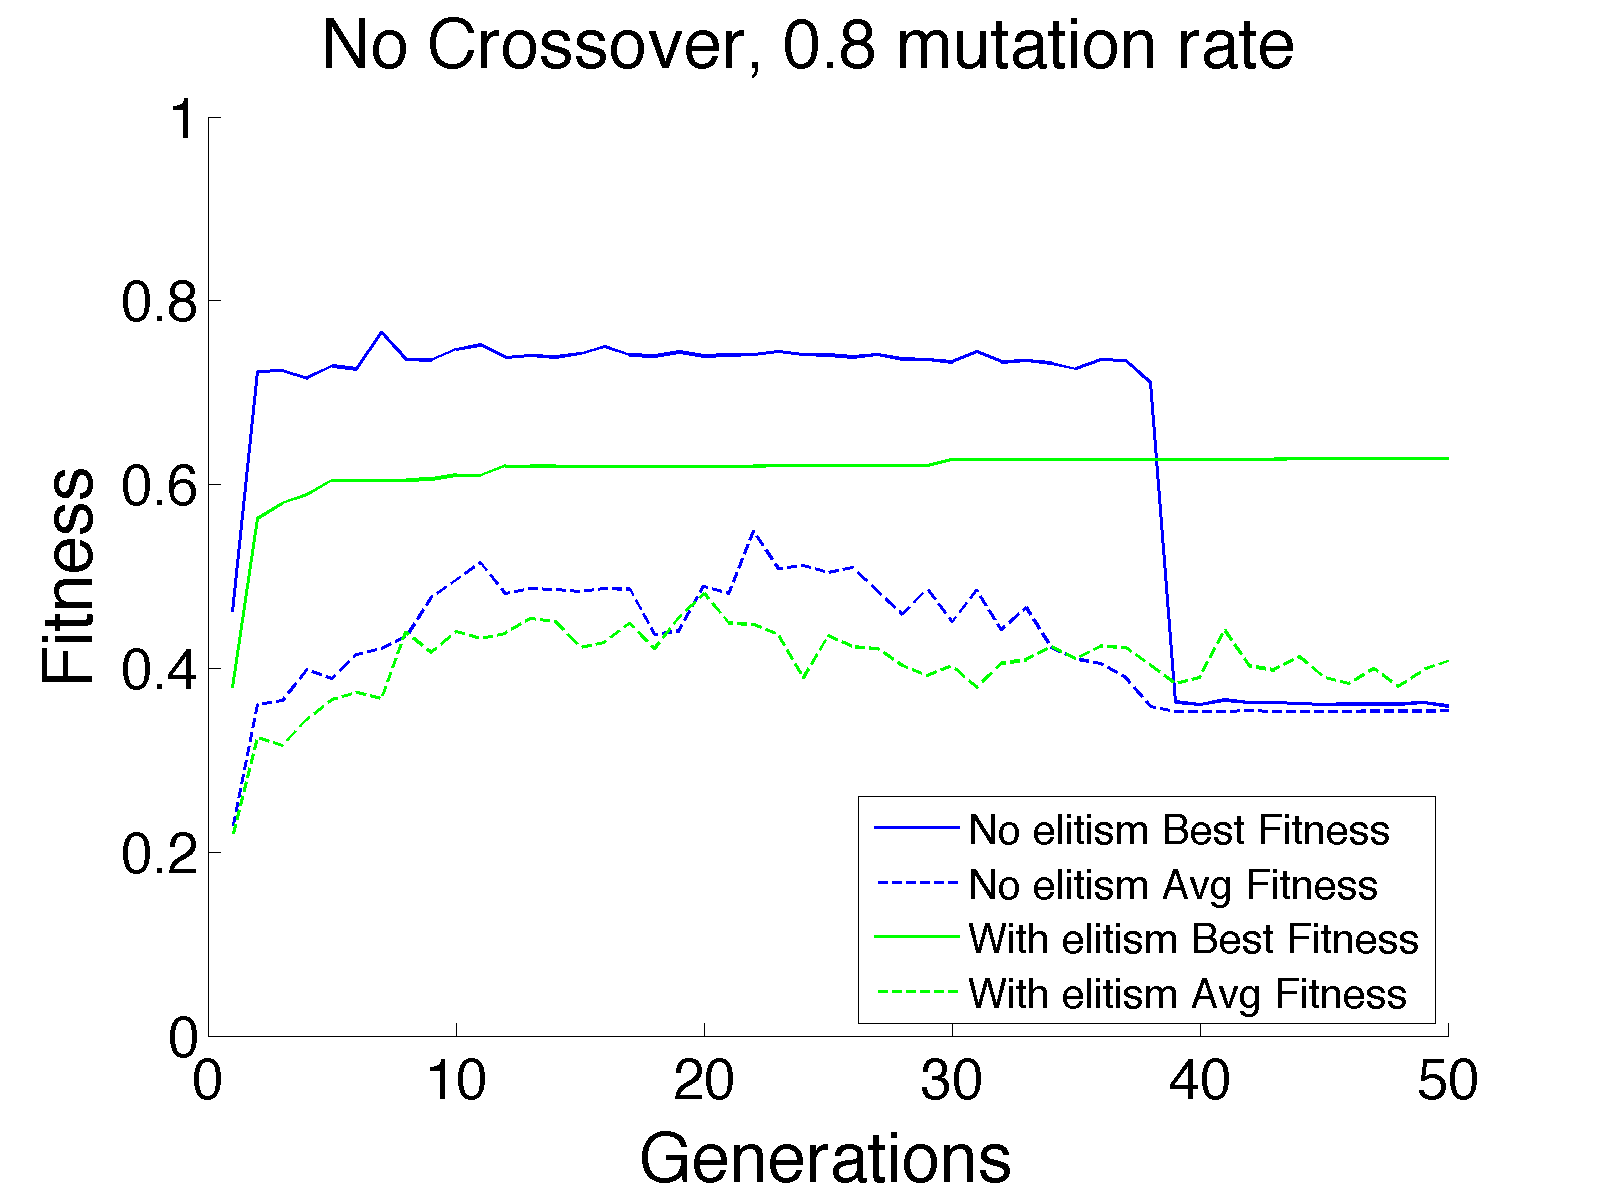
\includegraphics[width=0.6\textwidth,height=0.2\textheight]{figures/fitness08mut0crossDrop.png}
  \caption{Best and average fitness curves with and without elitism with no crossover and a 0.8 mutation rate. This figure highlights the danger in having a high mutation rate and no elitism.}
  \label{fig:fig4}  
\end{figure}

To tease out whether crossover or mutation was more important, we ran experiments with a high mutation rate and low crossover rate (See Figure ~\ref{fig:fig5}), and a high crossover rate and low mutation rate (See Figure ~\ref{fig:fig6}). 

\begin{figure}[H]
 \centering
  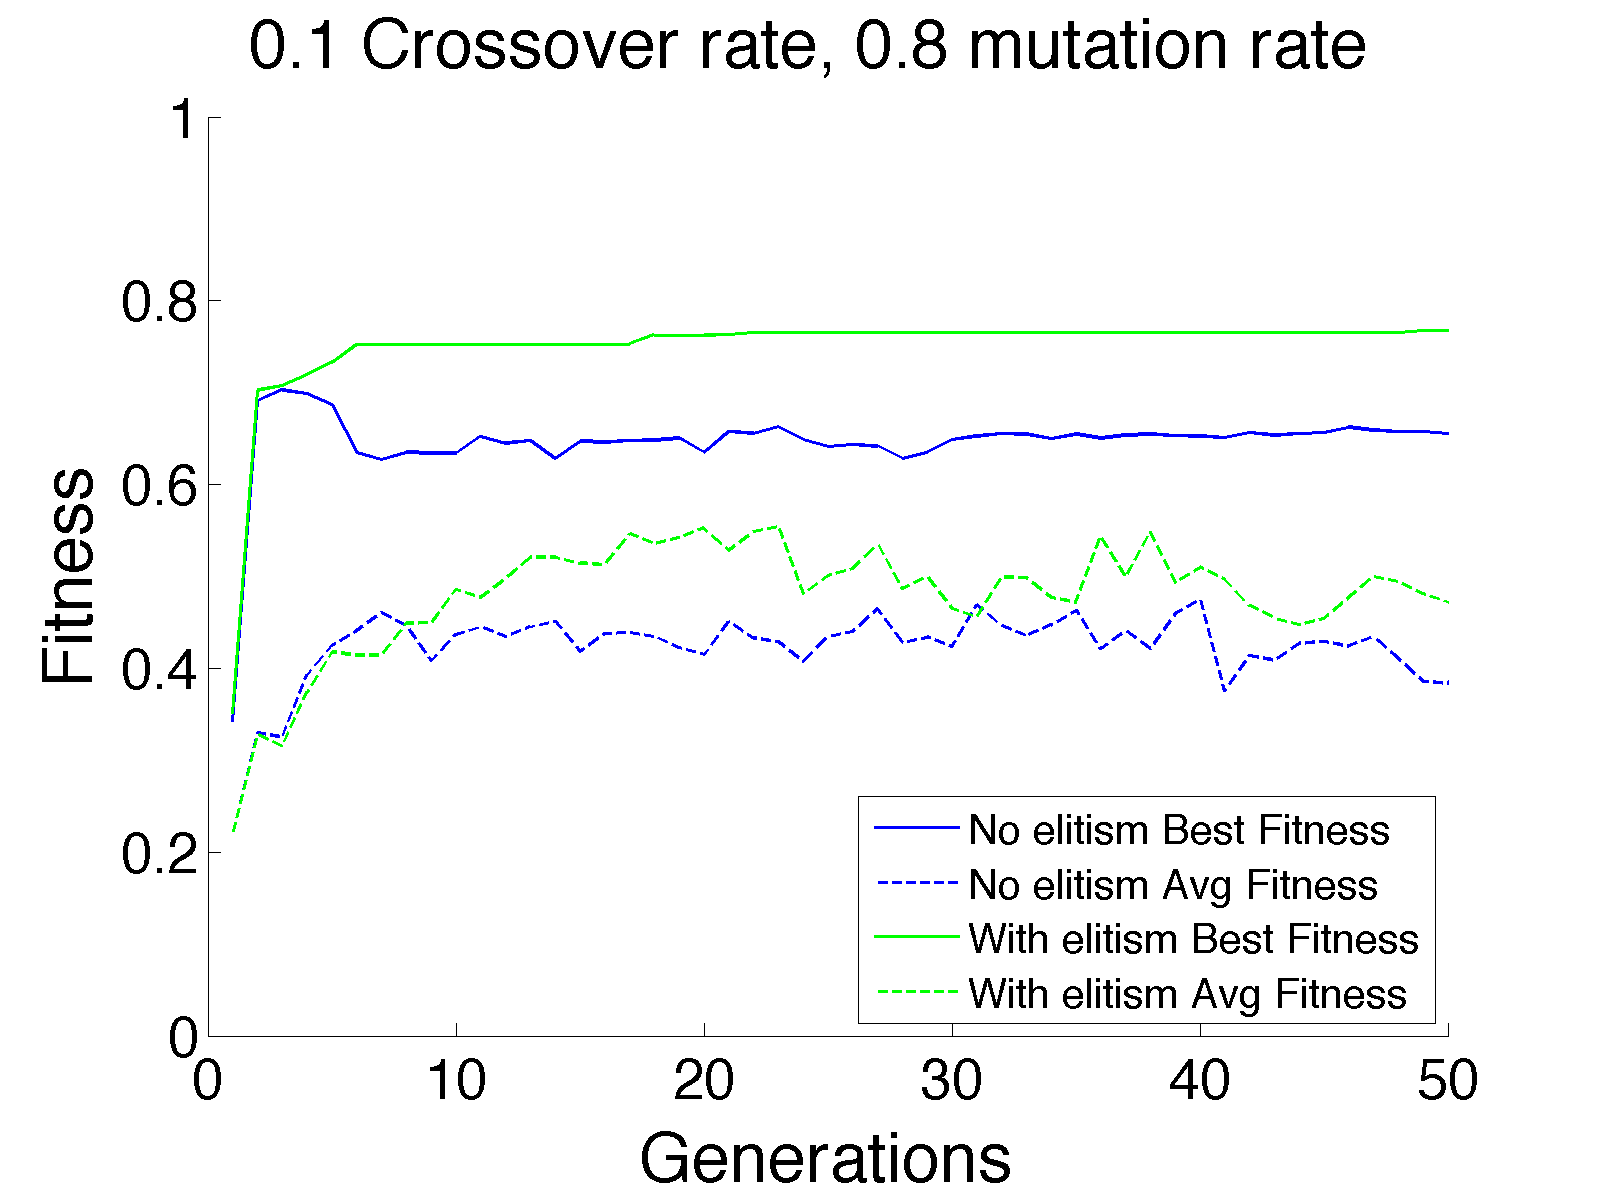
\includegraphics[width=0.6\textwidth,height=0.2\textheight]{figures/fitness08mut01cross.png}
  \caption{Best and average fitness curves with and without elitism with a 0.1 crossover rate and a 0.8 mutation rate}
  \label{fig:fig5}  
\end{figure}

\begin{figure}[H]
 \centering
  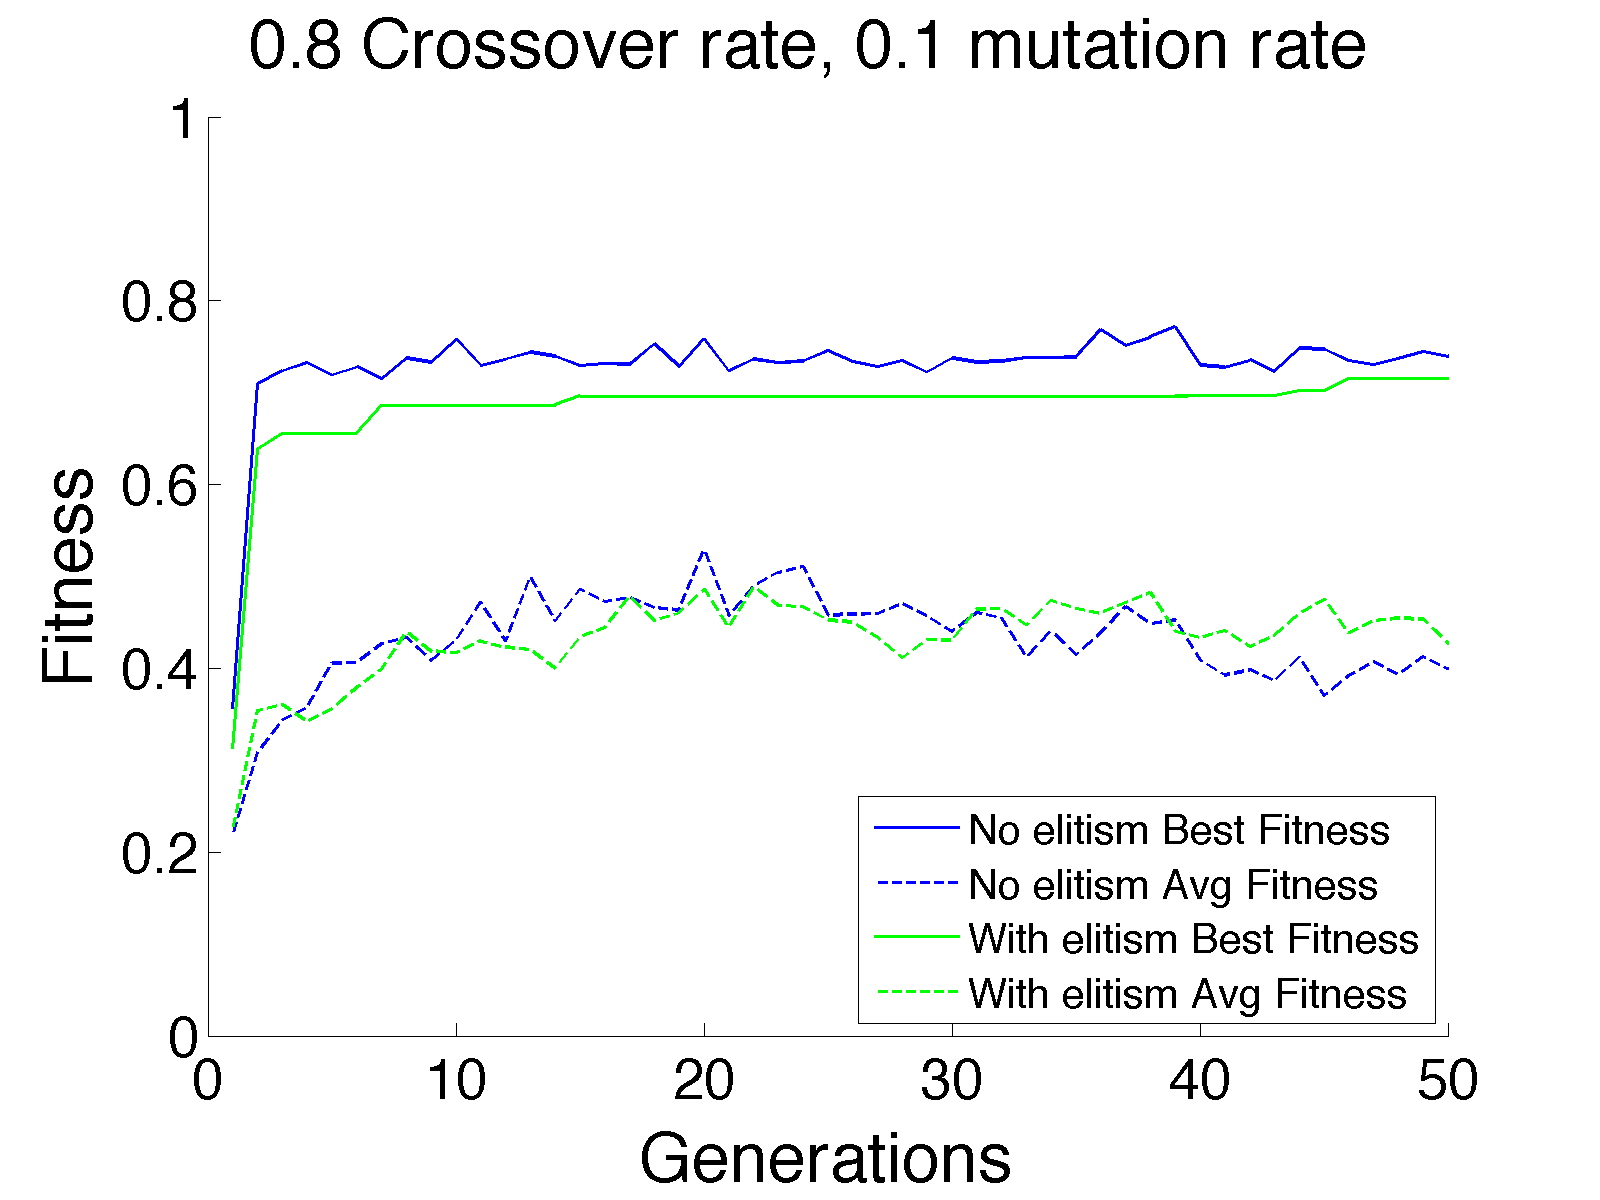
\includegraphics[width=0.6\textwidth,height=0.2\textheight]{figures/fitness01mut08cross.png}
  \caption{Best and average fitness curves with and without elitism with a 0.8 crossover rate and a 0.1 mutation rate}
  \label{fig:fig6}  
\end{figure}

These plots show very similar performance, although again we found that with a high mutation rate elitism is necessary, and with a high crossover rate but low mutation rate it is not.

The last experiment we did was plugging ithe parameters from our top-performing chromosome into Palacios VMM. Table~\ref{tab:table1} shows the resulting chrosome for that test case.

\begin{table}[H]
\centering
\begin{footnotesize}
\renewcommand{\arraystretch}{1.2}

 \begin{tabularx}{17cm}{ | X | X | X | X | X | X | X | X | X | X | X |}
 \hline
Machine ID & Fitness & TDF  & Phys. Core & PCore Speed (Khz) & Achieved Utilization & Max. Utilization & Virtual Core& VCore Speed (Khz) & Slice & Period \\ \hline

24 & 0.833 & 2 & 0 & 6198490 & 57.03 & 93 & 2 & 7742333 & 874929 & 1592000 \\ \hline
24 & 0.833 & 2 & 0 & 6198490 & 57.03 & 93 & 3 & 8115486 & 618205 & 1046012 \\ \hline

24 & 0.833 & 2 & 1 & 4922740 & 73.92 & 81 & 1 & 6731667 & 972710 & 1303450 \\ \hline
24 & 0.833 & 2 & 1 & 4922740 & 73.92 & 81 & 4 & 8866626 & 580009 & 792234 \\ \hline

24 & 0.833 & 2 & 2 & 6602449 & 87.61 & 90 & 0 & 2715879 & 438648 & 461707 \\ \hline
24 & 0.833 & 2 & 2 & 6602449 & 87.61 & 90 & 5 & 7215736 & 833966 & 1039601 \\ \hline

\end{tabularx}
\caption{Chromosome parameters for the test case with 3 physical cores and 6 virtual cores.} \label{tab:table1}
\end{footnotesize}
%\end{center}
\end{table}

Since a good fitness value of 0.83 was reached for this test case, we plugged this configuration into a guest virtual machine (VM) configuration file (XML configuration file included in turned in materials). The resulting virtual machine was launched in Palacios, which was able to allocate all the virtual cores correctly and run them on the physical CPUs (PalaciosLog.txt included in turned in materials). 

For the purposes of our work, the proper allocation of virtual cores over physical cores after the admission control phase in Palacios shows the correctness of the result. In additions to legal allocation, however, we also want good performance of the scheduler algorithm based on our allocation. After running the virtual machine for approximately 4 minutes, the log shows that all the virtual cores are scheduled periodically with a good performance. Table~\ref{tab:table2} shows the total time allocated to each virtual core during the time of the test. We can see that the CPU is shared properly among the virtual cores.

\begin{table}[H]
\centering
\renewcommand{\arraystretch}{1.2}

 \begin{tabularx}{275pt}{ | c | c | X | }
 \hline
Virtual Core ID & Physical Core ID & Total Time ($\mu$$s$) \\ \hline

0 & 0 & 27035047 \\ \hline

1 & 0 & 31594730 \\ \hline

2 & 1 & 37160840 \\ \hline

3 & 1 & 22056291 \\ \hline

4 & 2 & 22898879 \\ \hline

5 & 2 & 36099909 \\ \hline

\end{tabularx}
\caption{Total time allocated to each virtual core for EDF scheduler.}
 \label{tab:table2}
%\end{center}
\end{table}

\section{Conclusion}

In conclusion, we have written a functional genetic algorithm to evolve roughly optimal parameters for task allocation on real-time multiprocessors in preparation for EDF scheduling. This code works quickly and evolves functional allocation parameters for hundreds of virtual cores. We found that high mutation and crossover rates are not necessary for good performance, but that elitism is often critical when there is a high mutation rate. Future work for this project includes allowing standardizing the constraint function, so that allocations can be prepared for different types of tasks. Also, we would like to write code that allows for a best possible allocation, when more cores need to be scheduled than there is space for. Overall we are pleased at the performance of this genetic algorithm and hope to continue to work on it to transform it into a useful tool for task allocation on real-time multiprocessors.

\singlespacing
\bibliographystyle{abbrv}
\bibliography{finalProj_report}
\end{document}


